\documentclass[a4paper]{article}
\usepackage[letterpaper, margin=1in]{geometry} % page format
\usepackage{hyperref} % for urls
\def\UrlBreaks{\do\/\do-}
\usepackage{graphicx}
\usepackage{listings}
\usepackage{graphicx}
\graphicspath{ {} }


\title{Project - Network Intrusion Detection System\\CMPT469 Deep Learning w/ TensorFlow}
\author{Kai Wong}
\date{12/11/17}

\begin{document}

\maketitle

\section{Abstract}
\hspace*{10mm}This paper highlights the results of using a deep learning model for a network intrusion detection system (NIDS), implemented with a deep belief network made up of stacked RBMs and an RNN-LSTM architecture. With this architecture, a final average testing accuracy of 97.69\% was achieved, proving it to be an effective means for the connection classification problem.

\section{Introduction}
\hspace*{10mm}Cybersecurity is a major and pressing topic that all companies face in modern day. Building a reliable network intrusion detection system provides a great way to increase the security of a company's assets. By harnessing the power of deep learning through the use of neural networks, we can build a model that will accurately detect and classify the different types of attacks a network may face, and in turn better protect a company. For our data, we will use the NSL-KDDCup99 dataset, which is an improved version of the KDDCup99 dataset (cont. background/related work). The original KDDCup99 dataset, from the 1998 DARPA Intrusion Detection Evaluation Program, was created for the task of building a predictive model capable of distinguishing between bad connections (intrusions), and good connections (normal). The labeled dataset includes four main categories of attacks: denial-of-service (a flood of packets are sent such that computing/memory resources aren't available to serve authorized requests), user-2-root (the attempt to exploit susceptibilities in a system to achieve root privileges), probing (the attempt to examine a machine to determine susceptibility for exploitation), and remote-to-user (the attack in which an intruder sends packets to a machine to expose a machine’s vulnerabilities and achieve local user privileges); the goal is to classify an incoming connection as either normal or an attack and the attack type. In this dataset, the test data contains attack types not in training data, making this task more realistic, as intrusion experts believe that most novel attacks are variants of known attacks, and knowing the “signature” of known attacks can be sufficient to catch these novel attacks. Thus, the dataset contains 24 training attack types, with an additional 14 types in the test data only. The dataset comes with derived features that help in distinguishing normal connections from attacks.

\section{Background/Related Work in NIDs}
\hspace*{10mm}The majority of previous works demonstrate that building a model using a long short-term memory recurrent neural network yields great results on the KDDCup99 dataset. In this paper, we will go over a few of the past approached techniques in order to provide reasoning behind the architecture for our model.

\subsection{NSL-KDDCup99 Dataset}
\hspace*{10mm}The NSL-KDDCup99 dataset is an improved and reduced version of the KDDCup99 dataset [1]. The original dataset contained a lot of redundant records, both in the training and testing data, and this makes learning algorithms biased towards frequent attack records (i.e. DOS attacks in the KDDCup99 dataset), and leads to poor classification results for infrequent but harmful records. The NSL-KDD dataset eliminates these redundant records, and also partitions records into various classification difficulty levels (based on the number of learning algorithms that could correctly classify the records), then selecting records by random sample from each level. These steps of processing makes the number of records in the NSL-KDD dataset reasonable for the training of a learning algorithm [1].

\subsection{Auto-Encoders and Deep Auto-Encoders}
\hspace*{10mm}It can be seen how other deep learning approaches such as the use of auto-encoders can be beneficial in a network intrusion detection system (NIDS). In developing an effective and flexible NIDS for unknown future attacks, proper feature selection is key and difficult, as attack scenarios are continuously changing and evolving, and the features selected for one class of attack may not work well for other classes of attack [1]. In addition, producing a large labelled dataset from raw network traffic data collected over a period or in real-time is difficult. Therefore, the use of autoencoders can be helpful in providing automatic and meaningful feature extraction from unlabeled data [1,3] and also reducing the dimensionality of the data. A deep auto-encoder is simply an auto-encoder with multiple hidden layers, and has been used to train models on the NSL-KDD dataset [2, 5].

\subsection{Deep Belief Networks}
\hspace*{10mm}This notion of a neural network discovering patterns within data autonomously is a technique known as unsupervised learning, such as is done with the use of autoencoders. A deep belief network is made up of these autoencoders (or also with Restricted Boltzmann Machines (RBMs), and an algorithm greedily trains the network layer by layer using unsupervised learning [2]. Using this method provides a network that is successful in providing accurate classification for network intrusion detection [1,2].

\subsection{LSTMs and RNNs}
\hspace*{10mm}There are many previous works that have successfully built accurate learning algorithms using the feed-forward RNN-LSTM model [4,5,6,7]. It can be seen that anomaly detection models should be built to remember information from a number of previous events; a single data point in a collective data anomaly may not be considered to be an anomaly unless considered with the occurrences of other single points [4]. Thus, it can be seen that the ability to learn from historical data is important in a network intrusion detection model. This is what the RNN-LSTM model is capable of, and it is seen that extremely high classification accuracies are reported using this model [4,5,6,7].

\section{Methodology}
\hspace*{10mm}
We can see that the problem of network intrusion detection is a classification problem, as we need to be able to classify connections as either normal or the type of attack if it is an attack. With this in mind, and building off research previously done with network intrusion models, we can build an effective classification model by creating a deep belief network with a combination of Restricted Boltzmann Machines and a long short term memory recurrent neural network. 
\\\hspace*{10mm}
We will prepend the network with a layer of RBMs, which will reduce the dimensionality of the dataset and provide useful feature extraction. We will take the weights and biases produced here to better improve the training of the RNN-LSTM section of our model, as this pre-training has been shown to significantly decrease test error; pre-training allows the RNN-LSTM to not have to train from scratch, leading to better convergence and less test error. The use of an RNN-LSTM will allow the network to recognize patterns in the sequences of data passing through the network and retain memory, which offers advantages that were discussed in the previous past works section. Other transformations made to the data will include the transformation of the symbolic data columns into a one hot encoding vector. 
\\\hspace*{10mm}
The RBM portion of this model will be unsupervised, while the RNN-LSTM will be supervised.
9/10ths of the training data provided will be used in training, while the remaining 1/10th of the training data will be used for testing the accuracy of the model.
\\\hspace*{10mm}
The dataset, after data transformations, contains 122 features, with 23 different classes of attacks.
\\\hspace*{10mm}
After dimensionality is reduced by the layer of RBMs, the RNN-LSTM network will take the last RBM layer and use it as input, and will bring in the RBMs' weights and biases. It will perform $\sqrt{n}$ sequences of $\sqrt{n}$ points at a time, where n is the hidden units in last layer of RBM, such that it can fully learn the sequences of data points passing through the network.


\section{Experiments}
\subsection{Using a Shallow Neural Network Softmax Classifier versus an RNN-LSTM:}
\hspace*{10mm}
I wanted to see if there was an increase in accuracy when using an RNN-LSTM instead of a shallow neural network softmax classifier, to see the effectiveness of an RNN-LSTM.
\begin{center}
 \begin{tabular}{||c c c||} 
 \hline
Epoch &
Accuracy Rating for Shallow Neural Network Softmax Classifier &
Accuracy Rating for RNN-LSTM \\[0.5ex] \hline\hline
0 &
0.8328927627 &
0.9398 \\ 
 \hline
1 &
0.8684638772&
0.939133 \\ 
 \hline
2&
0.868455939&
0.931 \\ 
 \hline
3&
0.8684083097&
0.9404\\ 
 \hline
4&
0.8683527423&
0.946867\\ 
 \hline
5&
0.868344804&
0.947867\\ 
 \hline
6&
0.8683527423&
0.9395\\ 
 \hline
7&
0.8683686187&
0.943933\\ 
 \hline
8&
0.8683686187&
0.9482\\ 
 \hline
9&
0.8683686187&
0.9478\\ 
 \hline
10&
0.8683686187&
0.949767\\ 
 \hline
11&
0.8683686187&
0.9459\\ 
 \hline
12&
0.8683686187&
0.947567\\ 
 \hline
13&
0.8683686187&
0.9482\\ 
 \hline
14&
0.8683765569&
0.9449\\ 
 \hline
15&
0.8684003715&
0.948167\\ 
 \hline
16&
0.8684003715&
0.9457\\ 
 \hline
17&
0.8684003715&
0.938733\\ 
 \hline
18&
0.8684003715&
0.946\\ 
 \hline
19&
0.8684083097&
0.94723\\ 
 \hline
20&
0.8684083097&
0.946867\\ 
 \hline
21&
0.8684083097&
0.946267\\ 
 \hline
22&
0.8879124892&
0.9462\\ 
 \hline
23&
0.887904551&
0.945733\\ 
 \hline
24&
0.887904551&
0.946233\\ 
 \hline
\end{tabular}
\begin{figure}[h]
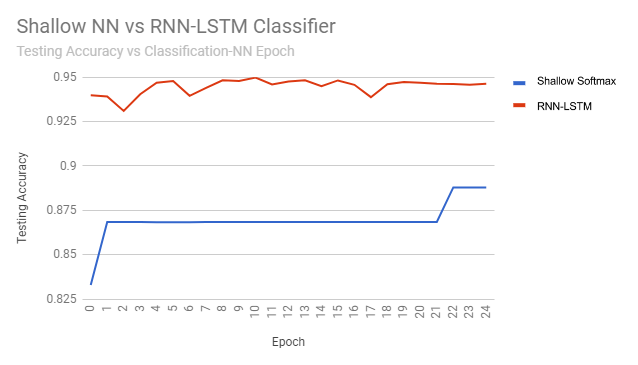
\includegraphics{shallowVsRnn}\caption{Shallow NN vs RNN-LSTM Classifier}\label{fig:XSS}
\end{figure}
\end{center}
\pagebreak
\subsection{Varying first layer of RBM:}
\hspace*{10mm}
I wanted to find the ideal number of hidden units in the first layer of the RBM. I figured that since the input had 123 features, a hidden unit size of 100 would be good to create a good representation of the data.\\
\hspace*{10mm}
I varied the number of hidden units in the first layer with the following: 50, 100, 150
\begin{center}
 \begin{tabular}{||c c c c||} 
 \hline
Epoch&
Accuracy Rating for 50 units&
Accuracy Rating for 100 units&
Accuracy Rating for 150 units\\[0.5ex] \hline\hline
0&
0.933&
0.940533&
0.9347\\ 
 \hline
5&
0.93367&
0.939933&
0.934833\\ 
 \hline
10&
0.9326&
0.946467&
0.9323\\ 
 \hline
15&
0.93303&
0.940733&
0.935733\\ 
 \hline
20&
0.9332&
0.942533&
0.9342\\ 
 \hline
25&
0.934567&
0.941867&
0.9359\\ 
 \hline
\end{tabular}
\begin{figure}[h]
\centering
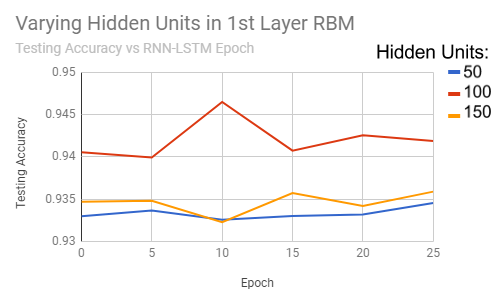
\includegraphics{varyRBM1st}\caption{Varying Hidden Units in 1st Layer RBM}\label{fig:XSS}
\end{figure}
\end{center}
\pagebreak
\subsection{Varying second layer of RBM:}
\hspace*{10mm}
I figured it would be best for the second layer of the RBM to be smaller than the first layer, as the job of the second layer is to extract features from the representation of the input.\\
\hspace*{10mm}
I varied the number of hidden units in the second layer with the following: 25, 36, 49
\begin{center}
 \begin{tabular}{||c c c c||} 
 \hline
Epoch&
Accuracy Rating for 25 units&
Accuracy Rating for 36 units&
Accuracy Rating for 39 units\\[0.5ex]\hline\hline
0&
0.9417&
0.9498&
0.943533\\ 
 \hline
5&
0.9521&
0.951767&
0.9567\\ 
 \hline
10&
0.9533&
0.960633&
0.9633\\ 
 \hline
15&
0.9543&
0.9609&
0.963\\ 
 \hline
20&
0.9548&
0.961767&
0.9651\\ 
 \hline
25&
0.954633&
0.961267&
0.968\\ 
 \hline
\end{tabular}
\begin{figure}[h]
\centering
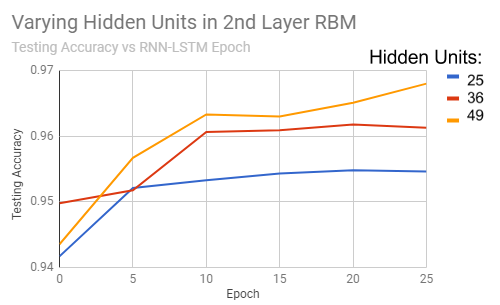
\includegraphics{varyRBM2nd}\caption{Varying Hidden Units in 1st Layer RBM}\label{fig:XSS}
\end{figure}
\end{center}
\pagebreak
\subsection{Varying epochs of RBM:}
\hspace*{10mm}
I wanted to find the best number of epochs to train the RBMs for in order to increase the overall testing accuracy of the network. I wanted to prevent overtraining of the RBMs.\\
\hspace*{10mm}
I varied the number of epochs the 2 layers of RBMs trained for 10 times with the following: 5, 25
\begin{center} \
 \begin{tabular}{||c c||} 
 \hline
Accuracy Ratings for 5 epochs&
Accuracy Ratings for 25 epochs\\[0.5ex]\hline\hline
0.97625&
0.970667\\ 
 \hline


0.972583&
0.964667\\ 
 \hline


0.98&
0.968417\\ 
 \hline


0.970667&
0.96875\\ 
 \hline


0.971667&
0.971\\ 
 \hline


0.973083&
0.972083\\ 
 \hline


0.97125&
0.96825\\ 
 \hline


0.9795&
0.972\\ 
 \hline


0.974167&
0.972417\\ 
 \hline


0.9755&
0.971083\\ 
 \hline


\end{tabular}
\pagebreak
\begin{figure}[h]
\centering
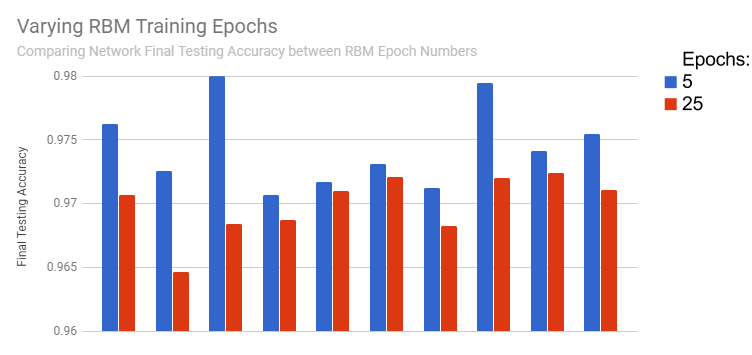
\includegraphics[width=6.5in]{varyRBMEpochs}\caption{Varying RBM Training Epochs}\label{fig:XSS}
\end{figure}
\end{center}
\subsection{Varying learning rate of RNN-LSTM:}
\hspace*{10mm}
I wanted find a good step size for the optimizer to traverse the cost function of the RNN-LSTM. I did not want the learning rate to be too big, as the step size would probably overshoot the minimum, but not too small, as I did not want the stuck local minima problem, or for the network to learn the detail too well and fail in generalization.
\\\hspace*{10mm}
I varied the learning rate of the RNN-LSTM with the following: 1, 0.1, 0.01, 0.001

\begin{center}
 \begin{tabular}{||p{3cm}|p{3cm}|p{3cm}|p{3cm}|p{3cm}||} 
 \hline


Epoch&
Accuracy Rating for Learning Rate of  1.0&
Accuracy Rating for Learning Rate of 0.1&
Accuracy Rating for Learning Rate of 0.01&
Accuracy Rating for Learning Rate of 0.001\\[0.5ex]\hline\hline
0&
0.3365&
0.940533&
0.9417&
0.9263\\
\hline
5&
0.535433&
0.940767&
0.9521&
0.9382\\
\hline
10&
0.830067&
0.943&
0.9533&
0.949033\\
\hline
15&
0.7943&
0.944133&
0.9543&
0.950833\\
\hline
20&
0.830067&
0.942167&
0.954033&
0.9516\\
\hline
25&
0.830067&
0.941867&
0.954633&
0.9516\\
\hline

\end{tabular}
\pagebreak
\begin{figure}[h]
\centering
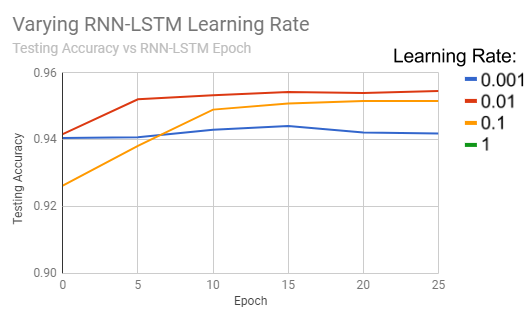
\includegraphics[width=5.5in]{varyLearnRNN}\caption{Varying RNN-LSTM Learning Rate}\label{fig:XSS}
\end{figure}
\end{center}


\section{Discussion and Analysis}
\subsection{Shallow Neural Network with Softmax Classifier vs RNN-LSTM Classifier:}
\hspace*{10mm}
Due to being a simple classifier, a shallow neural network does not have the power to have historical context in its learning or a concept of sequence learning. An attack may not seem like an attack out of context; a single point in a collective data anomaly may not seem like an anomaly. However, with context considered, the model learns to recognize an attack when considering a sequence of points, and it can learn long-term dependencies. This is exactly what an RNN-LSTM provides, and Figure 1 shows how it gives immediate better results when switching to it over a generic shallow neural network with softmax classification.
\subsection{Best parameters for the Deep Belief Network with RBMs and RNN-LSTM:}
\hspace*{10mm}
For the RBMs, a first layer of 100 hidden units and a second layer of 49 hidden units, with a learning rate of 1.0 and training over 5 epochs, produced the best results when combined with an RNN-LSTM hidden units size of 49, with a learning rate of 0.01 and training over 175 epochs.

\subsection{Best first layer of RBM:}
\hspace*{10mm}
A first layer RBM size of 100 gives the best final testing results.\\
\hspace*{10mm}
This seems to be due to the number of original features in the input data being 123. Therefore, an input layer of 100 creates a best representation of the input, as it is smaller than the input, but not by so much. A hidden layer of 50 is too small for a good overarching representation of the input to be created. A hidden layer of 150 and larger also causes testing error to increase, due to input not being compressed; here, the network learns the input too well. Even though the training accuracy of the RBMs lower, it causes the overall network to be bad at generalizing when it comes to testing. Figure 2 shows how a hidden units size of 100 is best for the first RBM layer.
\subsection{Best second layer of RBM:}
\hspace*{10mm}
A second layer RBM size of 49 gives the best final testing results.
\\\hspace*{10mm}
There are many factors that I think come into play here.
\\\hspace*{10mm}
First, in RBMs, subsequent hidden layers should be smaller than the first hidden layer. The first hidden layer had the job of creating a good overarching representation of the input; now the subsequent hidden layers have the job of being smaller such that the model is forced to better learn and extract hidden relationships from the initial representation of the data from the first layer.
\\\hspace*{10mm}
Due to the nature of how my model is implemented, the size of the last layer of the RBM becomes the number of hidden units in the RNN-LSTM. This is because the output from the last layer of the RBM is used as the input for the RNN-LSTM network.
\\\hspace*{10mm}
The more hidden units in an RNN-LSTM network, the more embedding that occurs (where the input is transformed into a vectorial representation for the network to learn from). Fewer hidden units means less embedding can occur; this, this causes the model to store less information about the information coming in. Therefore, more hidden units means more information for the RNN-LSTM to learn from, and thus it can make better classifications. Figure 3 shows how an increase in hidden units leads the testing accuracy of the network to improve.

\subsection{Best learning rate for RBM:}
\hspace*{10mm}
I did not bother varying the learning rate for the RBMs, as I was getting extremely good reconstruction errors for both layers (~0.01 for layer 1, ~0.006 for layer 2).
I know that the learning rate should not be too low for the first layer of the RBM, as the responsibility of the first layer is to learn a high level representation of the input; it should not learn the detail by using a smaller step size, otherwise the model will fail to generalize well and only learn to copy the input instead of abstracting it.

\subsection{Best epochs for RBM:}
\hspace*{10mm}
Training the RBM for 5 epochs gives the best final testing results.
\\\hspace*{10mm}
I think this has to do with overtraining the layers of RBMs. Originally, I had trained the stacked RBMs for 25 epochs, and I had gotten worse results than when training them with 5 epochs. Figure 4 shows the results of those tests. I got lower reconstruction rates when I trained them for 25 epochs as opposed to when I trained them for 5 epochs, but the final testing error of the network was higher. I can conclude that this caused the network to overfit slightly; it was learning the detail of the input too well in order to generalize well when encountering data it had never seen before.

\subsection{Best learning rate for RNN-LSTM:}
\hspace*{10mm}
A learning rate of 0.01 for the RNN-LSTM gives the best final testing results. 
\\\hspace*{10mm}
The network uses the AdamOptimizer (a better version of the GradientDescentOptimizer) which uses certain algorithms to control the learning rate, such as momentum, which improves convergence on the cost function. As can be seen in Figure 5, decreasing the learning rate from 1 to 0.01 improves final testing accuracy, meaning that in this cost function, a step size of 0.01 is able to find the minimum point in the cost function most effectively. Too big of a learning rate causes the optimizer to not find the minimum effectively, as it would keep “overshooting” it. Decreasing the learning rate from 0.01 to 0.001 decreases final testing accuracy, meaning that the step size is too small for the optimizer to find the global minimum in the cost function; it gets stuck in some local minimum, without finding the global minimum. Therefore, a learning rate of 0.01 is just right for this network.

\subsection{Best number of epochs for RNN-LSTM:}
\hspace*{10mm}A total number of about 175 epochs proved to give the best results for the RNN-LSTM. The network appears to not be negatively affected by large numbers of epochs; normally, this can lead a network to overfit, as it is being overtrained, and the network simply learns the input extremely well, failing to generalize in test cases. We can see in Figure 6, increasing the number of epochs to 150 leads to the network slowly seeing an increase in accuracy, until about 180 or so epochs, then it starts to waver or decrease, showing that this is probably where the network starts to overfit and where we should cut off training. Increasing the number of epochs allows the network to continually improve its classification abilities by adjusting its weights, and letting it continually do this for around 175 iterations gives it the ability to learn its best.

\subsection{Results of 10-fold cross validation:}
\hspace*{10mm}
I performed a 10-fold cross validation on my set; I trained on every 1/10th of the dataset, and trained on every other 9/10th of the dataset, for all 1/10ths of the dataset.
\hspace*{-20mm}
\begin{center}
\begin{tabular}{||p{2cm}|p{2cm}|p{2cm}|p{2cm}|p{2cm}|p{2cm}|p{2cm}||}
 \hline
Epoch&
Accuracy for 1st Fold&
Accuracy for 2nd Fold&
Accuracy for 3rd Fold&
Accuracy for 4th Fold&
Accuracy for 5th Fold&
Accuracy for 6th Fold\\[0.5ex]\hline\hline
0&
0.944083&
0.940083&
0.95475&
0.941&
0.94033&
0.94075\\\hline
25&
0.973667&
0.965417&
0.96525&
0.961&
0.963&
0.964833\\\hline
50&
0.974083&
0.9695&
0.965333&
0.9676&
0.965&
0.970083\\\hline
75&
0.975083&
0.969417&
0.96775&
0.969417&
0.966583&
0.97233\\\hline
100&
0.975417&
0.971833&
0.974417&
0.969917&
0.96925&
0.973083\\\hline
125&
0.976167&
0.97375&
0.979167&
0.97075&
0.971&
0.97325
\\\hline
150&
0.978&
0.974167&
0.979667&
0.971667&
0.969&
0.983083\\\hline
175&
0.97625&
0.972583&
0.98&
0.971583&
0.971667&
0.973083\\\hline
\end{tabular}
\hspace*{-2mm}\begin{tabular}{||p{2cm}|p{2cm}|p{2cm}|p{2cm}|p{2cm}|p{2cm}|p{2.5cm}||}
 \hline
 Epoch&
 Accuracy for 7th Fold&
Accuracy for 8th Fold&
Accuracy for 9th Fold&
Accuracy for 10th Fold&
Average Accuracy&
Standard Deviation\\[0.5ex]\hline\hline
0&
0.93733&
0.947083&
0.9355&
0.945667&
0.9426576&
0.004416719225\\\hline
25&
0.96425&
0.9695&
0.96975&
0.971083&
0.966775&
0.003307834518\\\hline
50&
0.969&
0.9755&
0.97125&
0.9725&
0.9699849&
0.002649270709\\\hline
75&
0.971&
0.97625&
0.972667&
0.973167&
0.9713664&
0.00241734306\\\hline
100&
0.971167&
0.977667&
0.974&
0.9745&
0.9731251&
0.001942564472\\\hline
125&
0.97325&
0.977&
0.97525&
0.975417&
0.9745001&
0.002335821296\\\hline
150&
0.973417&
0.978833&
0.974833&
0.977167&
0.9759834&
0.003812149094\\\hline
175&
0.9735&
0.9795&
0.974167&
0.99755&
0.9769883&
0.003376021307\\\hline

\end{tabular}
\pagebreak
\begin{figure}[h]
\centering
\hspace*{-5mm}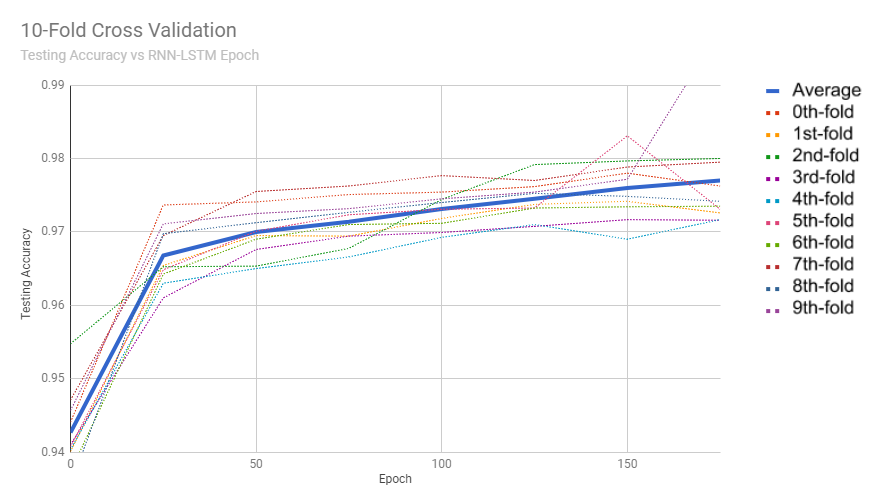
\includegraphics[width=7in]{10fold}\caption{10-Fold Cross Validation}\label{fig:XSS}
\end{figure}
\end{center}
\section{Conclusion}
\hspace*{10mm}
The goal of this paper was to create an effective network intrusion detection system with a neural network. We can conclude that using a deep belief network implemented with Restricted Boltzmann Machines and an RNN-LSTM classifier constructs an extremely effective network intrusion detection model, with a 97.69\% accuracy in classifying connections as normal or as malicious attacks. This paper shows how pre-training a network with RBMs leads to improving a model's convergence, as well as how using an RNN-LSTM allows a network to better classify sequences of data, which is especially important for network traffic. This will prove to be invaluable for companies looking to improve the security of their network and for other research groups looking to determine the significance of deep belief networks in anomaly detection. In the future, further work can be done to perhaps improve the network, such as adding another LSTM layer or including a dropout layer.


\section{References/Bibliography}
\hspace*{5mm}[1] Quamar Niyaz, Weiqing Sun, Ahmad Y Javaid, and Mansoor Alam, “A Deep Learning Approach for Network Intrusion Detection System”, \url{http://www.covert.io/research-papers/deep-learning-security/A%20Deep%20Learning%20Approach%20for%20Network%20Intrusion%20Detection%20System.pdf}

[2] Elike Hodo, Xavier Bellekens, Andrew Hamilton, Christos Tachtatzis and Robert Atkinson, “Shallow and Deep Networks Intrusion Detection System: A Taxonomy and Survey”, \url{https://arxiv.org/ftp/arxiv/papers/1701/1701.02145.pdf}

[3] Zhanyi Wang, “The Applications of Deep Learning on Traffic Identification”, \url{http://www.covert.io/research-papers/deep-learning-security/Applications%20of%20Deep%20Learning%20On%20Traffic%20Identification.pdf}

[4] Lo¨ıc Bontemps, Van Loi Cao, James McDermott, and Nhien-An Le-Khac, “Collective Anomaly Detection based on Long Short Term Memory Recurrent Neural Network”, \url{https://arxiv.org/ftp/arxiv/papers/1703/1703.09752.pdf}

[5] Manoj Kuma Putchala, “Deep learning approach for intrusion detection system (ids) in
the Internet of Things (IoT) network using Gated Recurrent Neural Networks (GRU)”,\\ \url{https://etd.ohiolink.edu/!etd.send_file?accession=wright1503680452498351&disposition=inline}

[6] Jihyun Kim, Jaehyun Kim, Huong Le Thi Thu, and Howon Kim, “Long Short Term Memory Recurrent Neural Network Classifier for Intrusion Detection”, \url{http://www.covert.io/research-papers/deep-learning-security/Long%20Short%20Term%20Memory%20Recurrent%20Neural%20Network%20Classifier%20for%20Intrusion%20Detection.pdf}

[7] Ralf C. Staudemeyer, “Applying long short-term memory recurrent neural networks to intrusion detection”, \url{http://sacj.cs.uct.ac.za/index.php/sacj/article/view/248/150}

\end{document}


